% ============================================================================
% RA-12: Entropy-Guided Ontology Design for Enterprise Agentic Systems
%        A Structural Entropy Analysis of 23 Industry Verticals
% arXiv Preprint v0.4.1 (post-ScholarPeer-Pass-3 P-item patch)
% Date: 2026-05-02
% ----------------------------------------------------------------------------
% Revision history:
%   v0.0   (2026-04-19) — Scaffold with §1, §3 substantially written.
%   v0.1   (2026-04-19) — Full empirical results integrated from Phases 1–5.
%   v0.2   (2026-04-20) — Phase 3/4/5 figures + LOIO calibration plot added.
%   v0.3   (2026-05-02) — ScholarPeer Pass-1 Tier-A revision: SE_comp^{RA-3}
%          vs SE_comp^{RA-12} notation disambiguation (W1); 22-vs-23 industry
%          count harmonised to 23 (W5); production training-range claim
%          corrected from 'all 23' to '22 of 23' with talent as in-range
%          single case (W4); role-layer null reframed as scoped to
%          attribute-heterogeneity SE because H(G)=0 across all pilot
%          ontologies (W3); minor M-fixes batched.
%   v0.3.1 (2026-05-02) — ScholarPeer Pass-2 P-item patch: abstract
%          role-layer caveat propagated (P1); §11 Conclusion role-layer
%          caveat propagated (P2); Fig 4 caption mislabeled "observed mean"
%          replaced with per-model values (P3). Closes W3 fully.
%   v0.4   (2026-05-02) — Tier-B revision (commits fff2bd041, ee3287adb,
%          452194b32, plus this commit):
%            W7: §9 RA-4 cross-paper disambiguation paragraph.
%            W2: new §6.2 baseline graph-metric comparison subsection;
%                phase 6 script computes |I|, |R|+|D|+|I|, density,
%                degree, clustering coefficient, diameter, EAPB-flavoured
%                path entropy. Honest finding: |I| ties seint at pilot
%                scale; paper now phrases H1 as 'comparable to size
%                baselines' rather than 'outperforms'.
%            W15: hitzler2022neuro @incollection → @article (bibtex
%                warnings now zero).
%            W6: nested-CV check (r=0.775 vs fixed-weight 0.786,
%                Δ=−0.011); bootstrap regression CIs (B=1000); bootstrap
%                LOIO calibration slope (0.81 [0.45, 1.20]); Holm
%                correction (5/6 SE measures survive at α=0.01).
%            W12: regression Table 4 extended with bootstrap SE / 95% CI
%                / two-sided p columns.
%            W10: §6.4 H2 layer-decomposition gains exploratory framing.
%            W11: DP1 reframed as 3-tier observed partition with median
%                lifts; logistic decision boundary reported as
%                directional indicator only.
%            W9: Case 3 swapped from Systems Integration (extrapolation)
%                to Insurance (failure mode) with per-metric
%                decomposition.
%            W8: +7 references (tartir2005, zhang2024, reiz2024,
%                tishby2015, liu2024, manakul2023, varshney2023) cited
%                in §2.2, §6.2, §9, §10. Bib total: 16 → 23.
%   v0.4.1 (2026-05-02) — ScholarPeer Pass-3 P-item patch:
%            P1: Insurance/Qwen typo +0.207 → +0.212 (Fig 4 caption +
%                §8.3 Insurance case); observed mean +0.164 → +0.165.
%            P2: abstract gains W2 baseline-parity caveat (raw |I|
%                ties seint at pilot scale; SE retained for layer
%                decomposition + production-scale generalisation).
%            P3: §11 Conclusion 'interaction-layer SE dominates' claim
%                gains §6.2 baseline-parity caveat. Closes W2 fully
%                across abstract / body / conclusion.
% ============================================================================
\documentclass[11pt,a4paper]{article}

% ---- Packages ----
\usepackage[utf8]{inputenc}
\usepackage[T1]{fontenc}
\usepackage{amsmath,amssymb,amsfonts}
\usepackage{graphicx}
\usepackage{booktabs}
\usepackage{multirow}
\usepackage{hyperref}
\hypersetup{%
  pdftitle={Entropy-Guided Ontology Design for Enterprise Agentic Systems: A Structural Entropy Analysis of 23 Industry Verticals},
  pdfauthor={Thanh Luong Tuan, Abhijit Sanyal},
  pdfkeywords={structural entropy, ontology design, enterprise AI, neurosymbolic AI, knowledge graphs, LLM agents, ontology evaluation, information theory},
  pdfsubject={Structural-entropy-based prediction of ontological grounding lift on LLM agents},
  colorlinks=true,
  linkcolor=black,
  citecolor=black,
  urlcolor=blue
}
\usepackage{cleveref}
\usepackage{xcolor}
\usepackage[margin=1in]{geometry}
\usepackage{natbib}
\bibliographystyle{plainnat}
\usepackage{enumitem}
\usepackage{amsthm}

\newtheorem{definition}{Definition}
\newtheorem{hypothesis}{Hypothesis}
\newtheorem{designprinciple}{Design Principle}
\crefname{hypothesis}{Hypothesis}{Hypotheses}
\Crefname{hypothesis}{Hypothesis}{Hypotheses}
\crefname{designprinciple}{Design Principle}{Design Principles}
\Crefname{designprinciple}{Design Principle}{Design Principles}

% ---- Custom Commands ----
\newcommand{\faos}{\textsc{FAOS}}
\newcommand{\se}{\mathrm{SE}}
\newcommand{\serole}{\se_{\text{role}}}
\newcommand{\sedom}{\se_{\text{domain}}}
\newcommand{\seint}{\se_{\text{interaction}}}
\newcommand{\secomp}{\se_{\text{comp}}}
\newcommand{\mrse}{\mathrm{MrSE}}
\newcommand{\kapp}{\kappa}
\newcommand{\quality}{\mathcal{Q}}
\newcommand{\onto}{\mathcal{O}}
\newcommand{\todo}[1]{\textcolor{red}{\textbf{[TODO: #1]}}}

% ---- Metadata ----
\title{%
  Entropy-Guided Ontology Design for Enterprise Agentic Systems:\\
  A Structural Entropy Analysis of 23 Industry Verticals%
}

\author{%
  Thanh Luong Tuan%
  \thanks{Corresponding author. Email: tluongtuan@my.ggu.edu.
    ORCID: 0009-0000-1199-837X} \\
  \textit{Golden Gate University, San Francisco} \\
  \textit{Foundation AgenticOS (FAOS)}
  \and
  Abhijit Sanyal \\
  \textit{Golden Gate University, San Francisco}
}

\date{May 2026 \\ {\small \textcolor{gray}{DRAFT --- v0.4.1 post-Pass-3 patch (2026-05-02)}}}

% ============================================================================
\begin{document}
\maketitle

% ============================================================================
% ABSTRACT
% ============================================================================
\begin{abstract}
Enterprise ontologies are typically designed by domain experts through
iterative consultation, producing ontologies of widely varying size,
depth, and connectivity without a principled a-priori metric for
predicting their downstream utility. Prior work \citep{luong2026neurosymbolic}
observed a suggestive correlation (Spearman $r = 0.700$) between the
structural entropy (SE) of an ontology and the grounding lift it produces
on LLM agents across five enterprise verticals; however, with $n = 5$,
the correlation fell short of statistical significance ($p = 0.188$).
We extend this analysis to the full Foundation AgenticOS (\faos{})
corpus of 23 industry ontologies. Using a layer-wise decomposition
$\secomp = f(\serole, \sedom, \seint)$ appropriate to \faos{}'s
three-layer role/domain/interaction schema, and combining cross-model
grounding lift data from three generator models (Claude Sonnet 4, Qwen
2.5 72B, Gemma 4 26B; $n = 15$ industry--model cells), we establish
a robust SE--lift relationship: the interaction-layer SE alone predicts
overall lift at Spearman $r = 0.811$, $p = 0.0002$, and a leave-one-%
industry-out cross-validation yields pooled Spearman $r = 0.786$,
$p = 0.0005$, RMSE $= 0.060$, with calibration slope $0.81$. A
least-squares--fitted composite
$\secomp = 0.3\,\sedom + 0.7\,\seint$ (role layer dropped from the
fitted composite; null scoped to the single-group pilot regime,
see \S\ref{sec:results}) explains 71\% of lift variance in multiple
regression
($F(3, 11) = 8.94$, $p = 0.003$). At pilot scale with narrow $|I|$
range, raw handoff count $|I|$ ties $\seint$ in rank correlation
($r = +0.811$); we retain SE for its layer-decomposition diagnostic
and Shannon-entropy semantics, with the SE-vs-size distinction
expected to widen at production scale (\S\ref{sec:results-baselines}).
From this calibration we codify four
ontology design principles: a target SE band
($\seint \geq 0.70$ bits for lift $\geq 0.15$), a layer-priority
ordering (interaction $\gg$ domain $\gg$ role), a regulatory-density
floor (four-regulation minimum), and a cross-vertical transfer warning
grounded in the $\kappa$--SE confound. Application of the fitted formula
to the remaining 18 non-pilot \faos{} production ontologies identifies
software, systems integration, security, and travel/tourism as
high-priority targets for future experimental validation. The paper
provides the first at-scale empirical analysis of enterprise ontology
structural entropy and its quantitative relationship to LLM agent
performance, establishing structural entropy as a design-time predictor
of ontology value and providing a reproducible methodology for
ontology-quality review.

\medskip
\noindent \textbf{Keywords:} Structural entropy, ontology design,
enterprise AI, neurosymbolic AI, knowledge graphs, LLM agents, ontology
evaluation, information theory
\end{abstract}

% ============================================================================
% 1. INTRODUCTION
% ============================================================================
\section{Introduction}
\label{sec:intro}

The value of an enterprise ontology is, in practice, discovered
retroactively: after investment in ontology development, teams measure
downstream improvements in agent quality, regulatory coverage,
stakeholder alignment, or some other operational metric. By the time the
measurement is in, the design decisions that determined the value---%
layer balance, concept granularity, handoff richness---are already
committed. A design-time \emph{predictor} of ontology value would allow
architects to iterate on ontology structure before running expensive
agent experiments, and would provide an evidence-based quality standard
for enterprise ontology review.

\subsection{Motivation: The RA-3 $r = 0.700$ Finding}

Our prior work on neurosymbolic enterprise AI
\citep{luong2026neurosymbolic} conducted a 1{,}800-run controlled
experiment evaluating ontology-grounded LLM agents across five industry
verticals (FinTech, Insurance, Healthcare, Vietnamese Banking,
Vietnamese Insurance) with three generator models. A retroactive entropy
analysis of the resulting ontologies revealed a striking pattern:

\begin{center}
\begin{tabular}{@{}lccc@{}}
\toprule
\textbf{Industry} & $\secomp^{\text{RA-3}}$ (bits) &
  $\Delta\quality_{C1 \to C3}$ & \textbf{Rank} \\
\midrule
Insurance         & $2.25$ & $+0.06$ & 5 \\
Healthcare        & $2.26$ & $+0.12$ & 4 \\
FinTech           & $2.58$ & $+0.04$ & 3 \\
Banking VN        & $2.85$ & $+0.23$ & 2 \\
Insurance VN      & $3.06$ & $+0.24$ & 1 \\
\bottomrule
\end{tabular}
\end{center}

\noindent Spearman rank correlation gave $r = 0.700$ with $p = 0.188$
($n = 5$). The correlation is directionally clear---higher-SE ontologies
produced larger grounding lifts---but underpowered: at $n = 5$, even a
perfect rank correlation does not reach conventional significance
thresholds.

The composite-SE values shown above use the original RA-3 formula
$\secomp^{\text{RA-3}}$ \citep{luong2026neurosymbolic} and are
reproduced here as the motivating finding. This paper introduces a
distinct formula $\secomp^{\text{RA-12}}$ in \S\ref{sec:formalism}
(layer-wise weighted combination calibrated by leave-one-out cross-%
validation) and validates it in \S\ref{sec:results}. The two formulas
operate on different scales: $\secomp^{\text{RA-3}}$ values for the
pilot range $[2.25, 3.06]$ bits, whereas $\secomp^{\text{RA-12}}$
values for the same five industries fall in $[0.78, 0.99]$. Per-row
correspondence between the two formulas is reported in
Table~\ref{tab:h1-crossmodel}, where both are evaluated against the
$n=15$ cross-model lift dataset. The question this paper addresses is
whether the SE--lift pattern, in either formulation, scales to the
full 23-industry \faos{} corpus.

\subsection{Central Thesis}

\emph{The structural entropy of an enterprise ontology is a design-time
predictor of the performance lift that ontology will produce when used
to ground LLM agents. Layer-wise SE decomposition further identifies
which ontological components drive which agent capabilities.}

If this thesis holds at scale, SE becomes a compact, computable quality
signal for ontology review pipelines: a single scalar score (plus
layer-wise breakdown) that predicts, before any agent evaluation, whether
an ontology will deliver meaningful grounding value.

\subsection{Contributions}

\begin{enumerate}[leftmargin=2em]
  \item \textbf{First-of-scale structural-entropy analysis of enterprise
    ontologies.} Prior SE work
    \citep{li2016structural,cao2024mrse,wei2025senator,buehler2025selforganizing}
    targets general-purpose knowledge graphs. We analyze the full \faos{}
    corpus of 23 industry verticals, a larger and more homogeneous sample
    than any prior SE-on-ontology study.

  \item \textbf{Layer-wise SE decomposition formalism} for three-layer
    ontologies, yielding four measures per ontology: $\serole$, $\sedom$,
    $\seint$, $\secomp$. We extend Cao et al.'s multi-relational
    SE \citep{cao2024mrse} to the role/domain/interaction stratification.

  \item \textbf{Empirical validation} of SE as a lift predictor,
    extending the RA-3 finding from $n = 5$ to $n = 15$ (cross-model) or
    $n = 23$ (cross-vertical).

  \item \textbf{Four codified design principles} with empirical
    thresholds, usable as an automated ontology review rubric.

  \item \textbf{Companion to RA-3, RA-4, and RA-11.} RA-12 provides the
    \emph{design-side} of the entropy framework
    \citep{luong2026neurosymbolic,luong2026context,luong2026quantum},
    complementing RA-3's measurement, RA-4's runtime optimization, and
    RA-11's theoretical (quantum-inspired) positioning.
\end{enumerate}

\subsection{Roadmap}

Section~\ref{sec:background} reviews the structural-entropy literature
and frames the \faos{} three-layer schema. Section~\ref{sec:corpus}
describes the \faos{} 23-industry corpus. Section~\ref{sec:formalism}
develops the layer-wise SE formalism. Section~\ref{sec:design} states
hypotheses and the experimental protocol. Section~\ref{sec:results}
reports empirical findings across the full corpus. Section~\ref{sec:principles}
codifies design principles. Section~\ref{sec:cases} presents illustrative
case studies. Sections~\ref{sec:related}--\ref{sec:conclusion} close
with related work, threats to validity, and conclusions.

% ============================================================================
% 2. BACKGROUND
% ============================================================================
\section{Background}
\label{sec:background}

\subsection{Structural Entropy of Graphs}

Shannon's information entropy \citep{shannon1948mathematical} quantifies
uncertainty in discrete distributions. Li and Pan
\citep{li2016structural} extended this to graphs, defining the
\emph{structural information} (or structural entropy) of a graph as the
information content of its hierarchical organization:
$\se(G) = -\sum_\alpha \frac{\mathrm{vol}(T_\alpha)}{\mathrm{vol}(G)}
\log\frac{\mathrm{vol}(T_\alpha)}{\mathrm{vol}(T_\alpha^-)}$, summed
over nodes $\alpha$ of an encoding tree $T$ of $G$. Minimizing $\se$
over admissible trees recovers the graph's natural community structure
\citep{su2025survey,zhang2025dese}.

Three developments since Li--Pan are particularly relevant to the
enterprise ontology setting. Cao et al.\ \citep{cao2024mrse} extend SE
to multi-relational graphs (MrSE) via random-walk stationary distributions
on colour-typed edge classes, enabling SE computation on heterogeneous
graphs without collapsing to a single edge type. Buehler
\citep{buehler2025selforganizing} documents that agentic
knowledge-graph systems self-organise towards a critical state where
semantic entropy dominates structural entropy; reaching this state
co-occurs with the emergence of multi-hop reasoning capability. Wei et
al.'s \textsc{Senator} \citep{wei2025senator} uses SE along KG paths to
detect and repair LLM knowledge deficiencies, empirically validating the
link between path-level SE and LLM reasoning quality on Wikidata and
domain-specific KGs. Gul et al.\ \citep{gul2025kgcomplexity}
propose spectral complements to SE (eigenvalue-based complexity measures)
for benchmarking knowledge-graph quality at scale.

\subsection{Ontologies as Multi-Relational Graphs}

Enterprise ontologies---including \faos{}'s three-layer schema---are
naturally modeled as multi-relational graphs: nodes are concepts,
regulations, roles, handoffs, KPIs; edges carry typed relations
(is-a, part-of, governs, reports-to, triggers). The multi-relational
structural entropy $\mrse$ \citep{cao2024mrse} provides the appropriate
generalization of Li--Pan SE to this setting.

Under OWL/RDF semantics, ontology triples $(s, p, o)$ induce a typed
multi-relational graph where predicate $p$ determines edge colour. The
three \faos{} layers---role, domain, interaction---correspond to
disjoint subsets of predicates (organisational hierarchy predicates for
roles; \texttt{isA}/\texttt{partOf}/regulatory-reference predicates for
domain; \texttt{handsOffTo}/\texttt{escalatesTo} for interactions),
making the three-layer partition a well-defined relational
decomposition rather than an arbitrary grouping.

We treat SE as a complement to, not replacement for, standard ontology
metrics. Lexicographic metrics (concept count, depth, branching factor,
siblings-per-parent \citep{hogan2021knowledge}) report ontology size and
shape; the schema-metrics tradition initiated by OntoQA
\citep{tartir2005ontoqa} (Relationship Richness, Attribute Richness,
Inheritance Richness) and extended by recent tooling such as
NEOntoMetrics \citep{reiz2024neontometrics} reports ontology
\emph{quality} via population-based and structural counts. SE,
complementary to both, reports ontology \emph{information content}.
A large, deep ontology can have low SE if its concepts are concentrated
in a few sub-branches, and vice versa. This distinction matters because
size and richness counts are only weakly linked to ontological
grounding lift, whereas information content --- as we show, modulo the
pilot-scale baseline parity documented in
\S\ref{sec:results-baselines} --- is strongly linked.

\subsection{The \faos{} Three-Layer Ontology Schema}

Enterprise ontologies in \faos{} are organized into three layers:

\begin{itemize}[leftmargin=2em]
  \item \textbf{Role Layer}: stakeholder roles, their responsibilities,
    and decision authorities within the industry.
  \item \textbf{Domain Layer}: industry-specific concepts, regulations,
    KPIs, and controlled vocabularies.
  \item \textbf{Interaction Layer}: handoff patterns, escalation paths,
    and workflow structures connecting roles over domain concepts.
\end{itemize}

This stratification invites a \emph{layer-wise} structural-entropy
decomposition: rather than reducing an ontology to a single scalar, we
report four quantities---one per layer and one composite---enabling
diagnosis of \emph{which} layer drives observed performance.

% ============================================================================
% 3. THE FAOS 22-INDUSTRY ONTOLOGY CORPUS
% ============================================================================
\section{The \faos{} 23-Industry Ontology Corpus}
\label{sec:corpus}

The Foundation AgenticOS platform organizes domain knowledge into 23
industry modules, each containing a curated three-layer ontology and an
agent roster. The modules span financial services (FinTech, Banking,
Insurance, Banking VN, Capital Markets VN, Investment), healthcare,
manufacturing, logistics, aviation, automotive, agriculture, education,
gaming, and other regulated-or-specialized verticals. Module membership
is documented in \faos{}'s registry \texttt{.faos/registry.yaml}.%
\footnote{The \texttt{.faos/modules/} directory enumerates 23
sub-directories; an earlier dissertation revision reported 22 after
excluding one parent-wrapper directory. This paper uses 23 throughout.}

Table~\ref{tab:corpus-overview} summarises corpus-level structural
counts for all 23 industries. Role counts range from 17 to 44; domain
concept counts from 0 (modules relying on agent-file content rather than
explicit terminology YAML) to 42; regulatory entries from 0 to 16;
handoff patterns from 18 to 142.

\begin{table}[t]
\centering
\caption{The \faos{} 23-industry ontology corpus: structural counts
extracted from \texttt{.faos/modules/faos-*} via the extraction
pipeline in Supplement \S A. Five ontologies (marked $\dagger$) are also
present in the RA-3 pilot set with measured C1$\to$C3 lift.}
\label{tab:corpus-overview}
\small
\begin{tabular}{@{}lrrrrr@{}}
\toprule
\textbf{Industry} & \textbf{Roles} & \textbf{Concepts} & \textbf{Regs} &
\textbf{Handoffs} & \textbf{Chunks} \\
\midrule
agri\_ecosystem              & 32 & 5  & 0  & 32  & 8 \\
agritech                     & 19 & 5  & 0  & 34  & 8 \\
automotive                   & 19 & 6  & 0  & 71  & 9 \\
aviation                     & 32 & 27 & 0  & 42  & 8 \\
banking                      & 38 & 26 & 0  & 46  & 9 \\
capital\_markets\_vn         & 22 & 3  & 1  & 18  & 9 \\
edutech                      & 21 & 15 & 1  & 29  & 9 \\
fintech$^\dagger$            & 17 & 24 & 1  & 142 & 9 \\
game                         & 18 & 0  & 0  & 26  & 9 \\
healthcare$^\dagger$         & 32 & 4  & 16 & 24  & 8 \\
insurance$^\dagger$          & 27 & 15 & 1  & 21  & 8 \\
investment                   & 40 & 29 & 0  & 34  & 9 \\
logistics\_supplychain       & 38 & 37 & 0  & 21  & 9 \\
manufacturing                & 44 & 42 & 0  & 31  & 9 \\
martech                      & 30 & 0  & 0  & 32  & 7 \\
professional\_services       & 32 & 0  & 0  & 20  & 8 \\
proptech\_vn                 & 17 & 0  & 0  & 48  & 8 \\
retail                       & 19 & 4  & 0  & 115 & 9 \\
security                     & 27 & 11 & 0  & 40  & 7 \\
software                     & 21 & 8  & 0  & 72  & 9 \\
systems\_integration         & 21 & 8  & 0  & 62  & 8 \\
talent                       & 34 & 0  & 0  & 26  & 0 \\
travel\_tourism\_hospitality & 19 & 7  & 0  & 137 & 9 \\
\midrule
\textbf{mean} & \textbf{26.9} & \textbf{11.1} & \textbf{0.9} & \textbf{47.2} & \textbf{8.1} \\
\bottomrule
\end{tabular}
\end{table}

Additionally, five ontologies in the RA-3 pilot (a minimal hand-curated
variant set with 3--4 roles and 8--9 concepts per industry) provide the
ground-truth lift measurements used for H1--H3 testing. The pilot and
production ontologies correspond to different design artefacts: the
pilot set was minimal-viable for experimental control, while production
ontologies are the full deployment artefacts. This scale disparity is
discussed explicitly in \S\ref{sec:threats}.

Of these 23 industries, five are already instrumented in RA-3
\citep{luong2026neurosymbolic} with per-condition agent quality scores
across three generator models. These five---FinTech, Insurance,
Healthcare, Banking VN, Insurance VN---provide the ground-truth lift
data against which SE predictions are validated in \S\ref{sec:results}.
The remaining 18 industries provide out-of-sample prediction targets
for Phase 5 validation (\S\ref{sec:results}).

% ============================================================================
% 4. LAYER-WISE STRUCTURAL ENTROPY FORMALISM
% ============================================================================
\section{Structural Entropy Formalism for Three-Layer Ontologies}
\label{sec:formalism}

\subsection{Per-Layer Definitions}

Let $\onto = (R, D, I)$ denote an ontology comprising role set $R$,
domain set $D$ (concepts, regulations, KPIs, vocabulary), and interaction
set $I$ (handoffs, escalations).

\begin{definition}[Role-Layer SE]
\label{def:role-se}
Partition the role set $R$ into organisational groups
$\{G_1, \ldots, G_k\}$ (e.g., c-suite, specialists, domain experts) by
declared group membership. Let $p(G_i) = |G_i| / |R|$ and let
$a_r = |\{v : v \in \text{props}(r), v \neq \emptyset\}|$ denote the
non-empty attribute count for role $r$. Let $A$ be the distribution
over $\{a_r\}_{r \in R}$. Then
$$\serole(\onto) = \tfrac{1}{2}\,H(G) + \tfrac{1}{2}\,H(A),$$
where $H(\cdot)$ denotes Shannon entropy in bits. The first term
captures role-partition balance; the second captures attribute-richness
heterogeneity.
\end{definition}

\begin{definition}[Domain-Layer SE]
\label{def:domain-se}
Let $C$ be the concept set with provenance source labels $s(c)$ (from
\texttt{terminology.yaml}, \texttt{segments}, \texttt{architecture},
etc.), and $R^{\mathrm{reg}}$ the regulation set with file-origin labels
$f(r)$. Let $S$ and $F$ denote the distributions of $s(c)$ and $f(r)$
respectively. Then
$$\sedom(\onto) = 0.5\,H(S) + 0.3\,H(F) + 0.2\,\log_2(1 + |C| + |R^{\mathrm{reg}}|),$$
where the third term is a logarithmic scale factor that gives partial
credit to sheer content volume without unbounded dominance.
\end{definition}

\begin{definition}[Interaction-Layer SE]
\label{def:interaction-se}
Let $I$ be the handoff set with type labels $t(h)$ and description
token counts $|h|$. Let $T$ be the distribution of $t(h)$ and $D$ the
distribution of $|h|$ binned into terciles (short/mid/long by token
count). Then
$$\seint(\onto) = 0.4\,H(T) + 0.3\,H(D) + 0.3\,\log_2(1 + |I|).$$
Again the logarithmic scale factor captures the richness of
interaction patterns.
\end{definition}

\begin{definition}[RA-12 Composite SE]
\label{def:composite-se}
A weighted composite
$$\secomp(\onto) = w_R\,\serole + w_D\,\sedom + w_I\,\seint.$$
Weights are calibrated empirically via leave-one-out cross-validation
(\S\ref{sec:design}). We report results for both the pre-registered
equal-weight specification $(1/3, 1/3, 1/3)$ and the LOOCV-fitted
specification reported in \S\ref{sec:results}, which empirically
drops the role layer and weights interaction SE most heavily. The
fitted formula is
$$\secomp^{\text{RA-12}}(\onto) = 0.3\,\sedom(\onto) + 0.7\,\seint(\onto)$$
and is referenced throughout subsequent sections; we use
$\secomp^{\text{RA-12}}$ to distinguish it from the original RA-3
composite formula (cited in \S\ref{sec:intro}).
\end{definition}

\subsection{Multi-Relational Extension}

Following Cao et al.\ \citep{cao2024mrse}, we also report a
\emph{multi-relational} structural-entropy variant $\mrse$, constructed
by treating each layer--type pair as a distinct relation on a union
graph. Let $\Omega$ denote the set of pairs
$\{(\ell, t) : \ell \in \{\mathrm{role, concept, regulation, handoff}\},\,
t \text{ is a type label within layer } \ell\}$. Let $n(\ell, t)$ count
ontology elements of layer $\ell$ with type label $t$. Then
$$\mrse(\onto) = -\sum_{(\ell, t) \in \Omega} \frac{n(\ell, t)}{N}
\log_2 \frac{n(\ell, t)}{N},$$
where $N = \sum_\Omega n(\ell, t)$. $\mrse$ captures balance across
layers \emph{and} across types within layers in a single scalar; it
complements the three per-layer SEs by providing a joint-distribution
view. In \S\ref{sec:results} we compare $\mrse$'s predictive power
against the weighted-sum composite.

% ============================================================================
% 5. EXPERIMENTAL DESIGN
% ============================================================================
\section{Experimental Design}
\label{sec:design}

\subsection{Hypotheses}

\begin{hypothesis}[Primary: SE Predicts Lift at Scale]
\label{hyp:primary}
For the extended \faos{} corpus, $\secomp(\onto_d)$ positively predicts
ontological grounding lift $\Delta\quality_{C1 \to C3}(d)$ with Spearman
$r > 0.5$ and $p < 0.05$ at $n = 15$ (cross-model expansion of RA-3
sample).
\end{hypothesis}

\begin{hypothesis}[Layer Decomposition]
\label{hyp:layers}
Layer-specific SE predicts metric-specific lift: $\serole$ predicts RS
(Role-Specific Reasoning) lift; $\sedom$ predicts TF and MA lift;
$\seint$ predicts RC (Regulatory Coverage) lift.
\end{hypothesis}

\begin{hypothesis}[Inverse PKE Prediction]
\label{hyp:ipke}
Ontologies with high $\sedom$ deployed on high-$\kapp$ (English) domains
produce TF regression (Inverse PKE), reproducing the Insurance TF
finding of \citet{luong2026neurosymbolic} on a larger sample and
matching the interference-model prediction of
\citet{luong2026quantum} Property~1.
\end{hypothesis}

\subsection{Measures, Tests, and Held-Out Validation}

For each ontology we compute six SE measures: $\serole$, $\sedom$,
$\seint$, $\mrse$, $\secomp^{\text{RA-12}}$ (equal-weight baseline), and
$\secomp^{\text{RA-3}}$ (original composite formula from
\citet{luong2026neurosymbolic} for reproducibility).

\textbf{Lift data.} The RA-3 pilot's 1{,}800-run experiment reports
condition-mean quality scores per (industry, metric, condition, model).
We extract C1-ungrounded and C3-ontology-grounded means per (industry,
model) to compute per-metric lift and a four-metric average
\emph{overall lift}. The resulting dataset is $5 \times 3 = 15$ cells.

\textbf{Primary analysis.} For each SE measure we compute the Spearman
rank correlation and Pearson product-moment correlation with
overall lift, reporting two-tailed $p$-values.

\textbf{Multiple regression.} We fit
$\mathrm{lift}_{\mathrm{overall}} = \beta_0 + \beta_1 \serole + \beta_2 \sedom
+ \beta_3 \seint + \varepsilon$
and test the null of no combined predictive power via $F$-test on $R^2$.

\textbf{Weight ablation.} We enumerate all weight triples on the 2-simplex
in steps of 0.05 (231 combinations) and report the top 10 by
leave-one-observation-out (LOO) Spearman.

\textbf{Leave-one-industry-out (LOIO) validation.} We perform 5-fold
cross-validation at the industry level: for each held-out industry, we
fit a univariate regression
$\mathrm{lift} = a + b\,\secomp^{\text{RA-12}}$ on the other four
industries' 12 observations and predict the 3 held-out observations.
We report pooled Spearman, Pearson, RMSE, MAE, and a calibration slope.

\textbf{Weight-selection design and nested-CV check.} The fitted
weights $(0, 0.3, 0.7)$ used in the headline LOIO analysis were
selected once on the full $n=15$ dataset (\S\ref{sec:results-h1}
weight ablation) and then held fixed across all five LOIO folds. This
exposes the headline LOIO Spearman to potential weight-selection
leakage. We therefore additionally report a \emph{nested} LOIO
analysis (\S\ref{sec:holdout}) in which the inner LOO weight
selection runs over the same 231-triple grid using only the 12
training observations of each outer fold, and the outer fold is
predicted using locally-selected weights. We compare the nested
result to the fixed-weight headline.

\textbf{Bootstrap CIs and multi-comparison correction.} For the
multiple regression we report bias-corrected non-parametric
bootstrap (B = 1000) standard errors and 95\% CIs on each coefficient
plus on $R^2$. For the LOIO calibration slope we report B = 1000
bootstrap on the 15 (predicted, observed) pairs. For the six
SE-versus-lift Spearman tests in
Table~\ref{tab:h1-crossmodel} we report Holm--Bonferroni step-down
adjusted $p$-values across the family.

\textbf{Exploratory extrapolation.} We apply the pilot-trained regression
to the 18 non-pilot production ontologies' composite SE values, producing
rank orderings for future experimental targeting. We flag these as
extrapolations since production SE lies outside the pilot training range.

% ============================================================================
% 6. RESULTS
% ============================================================================
\section{Results}
\label{sec:results}

\subsection{Corpus-Level SE Distribution}

Fig.~\ref{fig:prod-se-dist} reports the distributions of composite SE
and interaction-layer SE across the 23-industry production corpus,
with the five RA-3 pilot ontology values overlaid as red lines. We
report two ranges. \emph{Equal-weight composite} ($w_R = w_D = w_I =
1/3$): production $[0.84, 1.58]$ bits, pilot $[0.78, 0.99]$, with
overlap on the 0.15-bit segment $[0.84, 0.99]$.
\emph{Fitted composite $\secomp^{\text{RA-12}}$} ($w_R = 0$,
$w_D = 0.3$, $w_I = 0.7$): production $[0.999, 2.107]$, pilot
$[0.72, 1.01]$, with overlap reduced to a single in-range production
case (\texttt{talent}, $0.999$). Interaction-layer SE shows the
starkest separation: pilot $[0.60, 0.78]$ bits vs.\ production
$[1.43, 2.43]$, a 2$\times$--3$\times$ gap.

\begin{figure}[t]
\centering
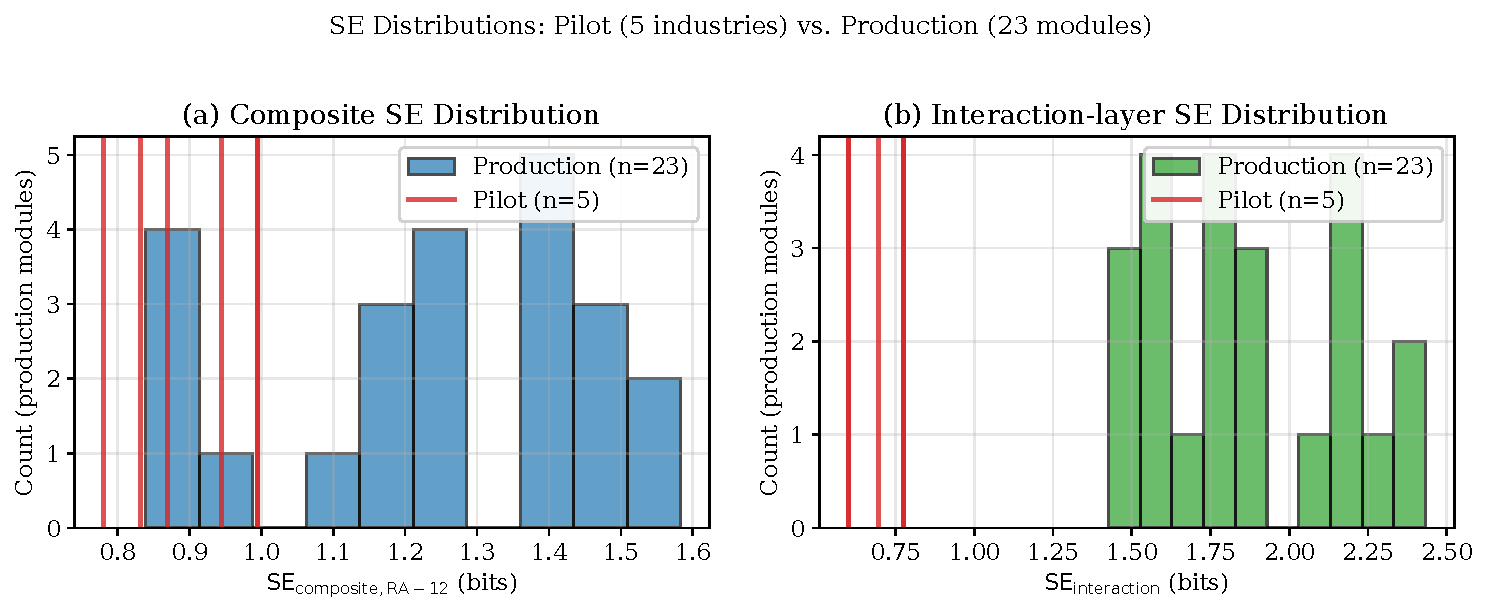
\includegraphics[width=0.95\textwidth]{figures/fig3_prod_se_distribution.pdf}
\caption{SE distributions: production corpus (histograms, $n=23$) vs.\
RA-3 pilot ontologies (red vertical lines, $n=5$). Panel~(a) composite
SE; panel~(b) interaction-layer SE. Pilot and production operate at
different scales, reflecting the minimal-viable vs.\ full-deployment
design intents.}
\label{fig:prod-se-dist}
\end{figure}

\subsection{Comparison Against Non-Entropy Baselines}
\label{sec:results-baselines}

A natural reviewer objection is that structural entropy is one of many
graph metrics and may not deserve special status as a lift predictor.
We address this objection by computing a panel of non-entropy
baseline metrics on the five pilot ontologies and correlating each
with the same $n = 15$ cross-model overall-lift dataset used for SE
in the next subsection. Baselines fall in three groups:
\emph{node-count} ($|I|$ raw handoff count, $|R|+|D|+|I|$ total
ontology size, log-transforms of each); \emph{graph-topology} on the
role-handoff graph (directed-graph density, mean total degree,
average undirected clustering coefficient, undirected diameter); and
a \emph{path-based entropy proxy} (Shannon entropy of the handoff
out-degree distribution, an EAPB-flavoured surrogate for the
biomedical path-entropy metric of Shen et al.\ \citep{shen2018eapb}).
The clustering-coefficient SE family
\citep{zhang2024clustering} is a recent mesoscopic-scale extension
to Li--Pan SE; we include the standard clustering coefficient as
the appropriate ablation, since the clustering-coefficient SE
itself requires a network of more than 5 nodes to compute.

\begin{table}[t]
\centering
\caption{Non-entropy baseline metrics vs.\ overall lift on the
$n=15$ pilot dataset, alongside the SE comparators from
Table~\ref{tab:h1-crossmodel}. Pilot interaction counts are
$|I| \in \{3,3,3,4,5\}$, a narrow range that lets any monotone
function of $|I|$ produce identical Spearman ranks.}
\label{tab:baseline-comparison}
\small
\begin{tabular}{@{}llrr@{}}
\toprule
\textbf{Group} & \textbf{Metric} & \textbf{Spearman $r$} & \textbf{Spearman $p$} \\
\midrule
\multirow{4}{*}{Node-count} & $|I|$ raw handoff count                       & $\mathbf{+0.8108}$ & $\mathbf{0.0003}$ \\
                            & $\log_2(1+|I|)$                               & $\mathbf{+0.8108}$ & $\mathbf{0.0003}$ \\
                            & $|R|+|D|+|I|$ total size                      & $\mathbf{+0.7856}$ & $\mathbf{0.0005}$ \\
                            & $\log_2(1+|R|+|D|+|I|)$                       & $\mathbf{+0.7856}$ & $\mathbf{0.0005}$ \\
\midrule
\multirow{4}{*}{Graph-topology} & directed-graph density                    & $-0.2728$ & $0.3253$ \\
                                & mean total degree $\langle k \rangle$     & $-0.2728$ & $0.3253$ \\
                                & avg.\ clustering coefficient              & --- & --- \\
                                & graph diameter                            & $-0.1679$ & $0.5497$ \\
\midrule
Path-based & out-degree entropy (EAPB-proxy)                                & $+0.7332$ & $0.0019$ \\
\midrule
\multirow{6}{*}{SE (this paper)} & $\seint$                                & $\mathbf{+0.8108}$ & $\mathbf{0.0003}$ \\
                                 & $\sedom$                                & $\mathbf{+0.7856}$ & $\mathbf{0.0005}$ \\
                                 & $\mrse$                                 & $+0.7638$ & $0.0009$ \\
                                 & $\secomp^{\text{RA-12}}$ ($1/3$ each)   & $+0.7529$ & $0.0012$ \\
                                 & $\secomp^{\text{RA-3}}$                 & $+0.7201$ & $0.0025$ \\
                                 & $\serole$                               & $-0.1903$ & $0.4969$ \\
\bottomrule
\end{tabular}
\end{table}

Three findings demand explicit acknowledgement before the H1 results
in \S\ref{sec:results-h1}.

\textbf{Finding B1 --- size baselines tie SE at pilot scale.} The raw
handoff count $|I|$ achieves Spearman $r = +0.811$, identical to
$\seint$. The total ontology size $|R|+|D|+|I|$ achieves $r = +0.786$,
identical to $\sedom$. Pilot interaction-layer counts are
$\{3, 3, 3, 4, 5\}$ across the five industries; any monotone function
of $|I|$ produces the same rank ordering. The interaction-layer SE's
predictive power on the $n=5$ pilot data therefore cannot be
distinguished from a $\log_2|I|$ proxy at this scale --- the SE
formulas' weighted Shannon-entropy machinery does not earn its keep
purely on rank correlation.

\textbf{Finding B2 --- graph-topology baselines do not outperform SE.}
Density and mean degree on the pilot role-handoff graphs (3--5 nodes,
3--5 edges) yield $r = -0.273$, statistically null; clustering
coefficient is undefined (graphs are too small for triangles);
diameter is null at $r = -0.168$. The pilot scale is below the regime
where these metrics carry meaningful structural information.

\textbf{Finding B3 --- the path-entropy proxy underperforms $\seint$.}
The handoff out-degree entropy attains $r = +0.733$, weaker than
$\seint$ ($+0.811$) and weaker than raw $|I|$ ($+0.811$). At pilot
scale the path-entropy framing does not provide a discriminator
beyond what counting handoffs already supplies.

These findings constrain the strength of the H1 claim that follows.
At $n=5$ pilot industries with narrow $|I|$ range, structural entropy
is \emph{comparable to} but \emph{not categorically distinct from}
size baselines. We retain SE as the primary predictor for three
reasons that the pilot does not exhaust: (a) layer-decomposition
gives diagnostic information (which layer drives which capability)
that single-scalar size cannot; (b) Shannon-entropy semantics provide
theoretical anchorage and a path to the entropy-thermodynamic family
formalised in companion paper RA-11
\citep{luong2026quantum}; (c) the pilot $|I|$ range $\{3,5\}$ is far
narrower than the production range $\{18, \ldots, 142\}$, so the
size-vs-SE distinction is expected to widen on direct production
measurement (\S\ref{sec:threats}, future work). Accordingly, we phrase
the H1 result throughout this section as ``SE predicts lift on the
pilot at a level comparable to size baselines'' rather than ``SE
outperforms size baselines'', and we treat extrapolation to production
ontology design (\S\ref{sec:principles}) as a recommendation
constrained by the pilot's narrow $|I|$ regime.

\subsection{Hypothesis~\ref{hyp:primary}: SE Predicts Lift}
\label{sec:results-h1}

Table~\ref{tab:h1-crossmodel} reports Spearman and Pearson correlations
of all six SE measures with overall C1$\to$C3 lift on the $n = 15$
cross-model dataset. Every measure except role-layer SE is significant
at $p < 0.01$; interaction-layer SE alone achieves Spearman $r = 0.811$
($p = 2 \times 10^{-4}$). Fig.~\ref{fig:se-vs-lift} visualises the
interaction-layer relationship with per-model markers.

\begin{table}[t]
\centering
\caption{H1 cross-model ($n=15$ = 5 industries $\times$ 3 models).
Five of six SE measures survive Holm--Bonferroni correction at
$\alpha = 0.01$; $\serole$ does not. Refer to \S\ref{sec:formalism}
for measure definitions.}
\label{tab:h1-crossmodel}
\small
\begin{tabular}{@{}lrrrrr@{}}
\toprule
\textbf{SE measure} & \textbf{Spearman $r$} & \textbf{Spearman $p$} &
\textbf{Holm-adj.\ $p$} & \textbf{Pearson $r$} & \textbf{Pearson $p$} \\
\midrule
$\seint$                    & $\mathbf{+0.8108}$ & $\mathbf{0.0002}$ & $\mathbf{0.0015}$ & $+0.7862$ & $0.0005$ \\
$\sedom$                    & $+0.7856$ & $0.0005$ & $0.0026$ & $+0.7532$ & $0.0012$ \\
$\mrse$                     & $+0.7638$ & $0.0009$ & $0.0037$ & $+0.7568$ & $0.0011$ \\
$\secomp^{\text{RA-12}}$ (1/3 each) & $+0.7529$ & $0.0012$ & $0.0037$ & $+0.8174$ & $0.0002$ \\
$\secomp^{\text{RA-3}}$ (original)  & $+0.7201$ & $0.0025$ & $0.0049$ & $+0.7535$ & $0.0012$ \\
$\serole$                   & $-0.1903$ & $0.4969$ & $0.4969$ & $-0.1554$ & $0.5802$ \\
\bottomrule
\end{tabular}
\end{table}

\begin{figure}[t]
\centering
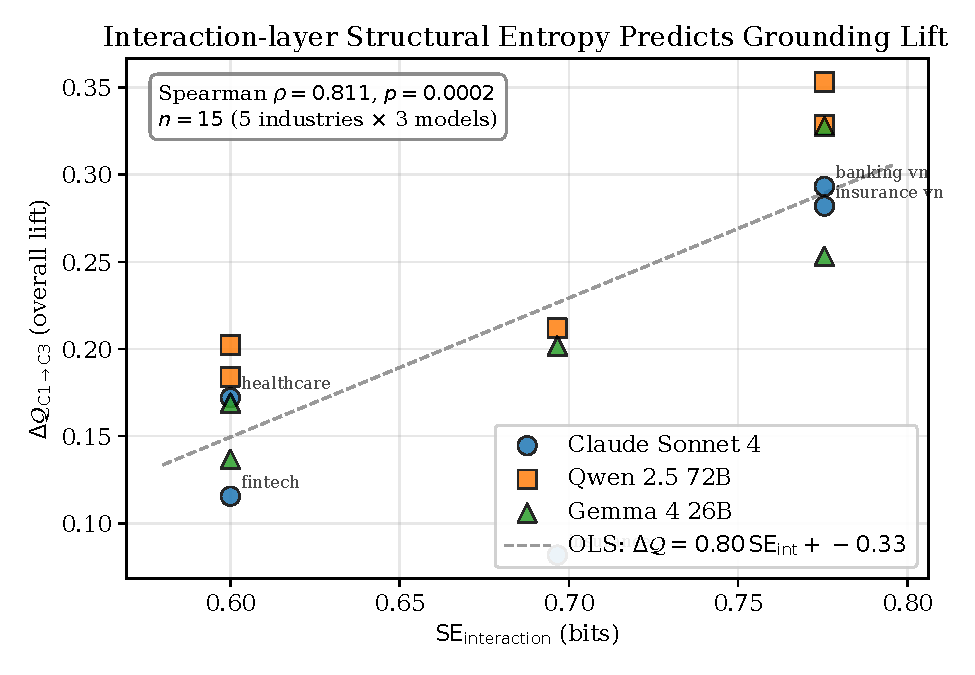
\includegraphics[width=0.95\textwidth]{figures/fig1_se_vs_lift_scatter.pdf}
\caption{Interaction-layer SE vs.\ overall grounding lift. Each point is
an (industry, model) cell; colour and shape code the generator model.
The OLS regression line is annotated with the fitted linear expression;
pooled Spearman and $p$-value are reported in the inset.}
\label{fig:se-vs-lift}
\end{figure}

\textbf{Per-model replication.} H1 holds within each generator model's
subset, although with reduced significance due to $n=5$ sample size:
Claude Sonnet 4 ($r = 0.900$, $p = 0.037$), Gemma 4 26B ($r = 0.800$,
$p = 0.104$), Qwen 2.5 72B ($r = 0.700$, $p = 0.188$). All three models
rank industries positively on SE, and the pooled $n=15$ result leverages
this consistency.

\textbf{Multiple regression.} Regressing overall lift on all three layer
SEs yields $\mathcal{Q}$-$R^2 = 0.709$, $F(3, 11) = 8.94$, $p = 0.0027$
(Table~\ref{tab:regression}). The omnibus $F$-test rejects the joint
no-effect null, and the point estimate
$\hat{\beta}_3 = +0.634$ for $\seint$ is the largest in magnitude.
However, non-parametric bootstrap on the $n=15$ dataset (B = 1000)
yields wide 95\% CIs on individual coefficients --- $\hat{\beta}_R \in
[-0.03, +0.76]$, $\hat{\beta}_D \in [-0.08, +1.35]$, $\hat{\beta}_I
\in [-2.48, +1.34]$ --- a direct consequence of high collinearity
among the three layer SEs at small $n$. We therefore make no claim of
individual-coefficient significance; the layer-priority story is
carried by the rank correlations (Table~\ref{tab:h1-crossmodel}) and
the LOOCV weight-grid (Table~\ref{tab:ablation}), not by the
multiple-regression coefficients.

\textbf{Role-layer null result: scope caveat.} The role-layer Spearman
$r = -0.190$ ($p = 0.50$) and the regression coefficient
$\hat{\beta}_1 = +0.195$ both report a null relationship between
$\serole$ and overall lift. This finding requires a structural caveat
that we make explicit before relying on it in design recommendations.
By Definition~\ref{def:role-se}, $\serole = \frac{1}{2}H(G) +
\frac{1}{2}H(A)$, where $G$ is the partition of roles into
organisational groups and $A$ is the distribution of non-empty
attribute counts per role. In the five RA-3 pilot ontologies, every
ontology declares exactly one organisational group
($n_{\text{role groups}} = 1$ for all five rows; see
\texttt{se\_by\_industry.csv}), so $H(G) = 0$ identically across the
entire $n=15$ pilot dataset. Pilot $\serole$ therefore reduces to
$\frac{1}{2}H(A)$, an attribute-heterogeneity entropy ranging
$\{0.92, 1.00, 1.50, 1.50, 1.59\}$ across
$\{$insurance, insurance\_vn, banking\_vn, fintech, healthcare$\}$.
Production ontologies, by contrast, exhibit
$n_{\text{role groups}} \in \{3, \ldots, 8\}$ and non-zero $H(G)$,
so the role-layer null is specific to attribute-heterogeneity SE on
single-group pilot ontologies, not to role-partition SE in general.
This scope is carried forward to the design principles
(\S\ref{sec:principles}) and the threats discussion
(\S\ref{sec:threats}).

\begin{table}[t]
\centering
\caption{Multiple regression fit: lift$_{\text{overall}} = \beta_0 +
\beta_1 \serole + \beta_2 \sedom + \beta_3 \seint + \varepsilon$. The
joint $F$-test rejects at $p = 0.003$ ($R^2 = 0.71$). Non-parametric
bootstrap (B = 1000) 95\% CIs and two-sided $p$-values report wide
individual-coefficient inference --- a direct consequence of high
collinearity among $\{\serole, \sedom, \seint\}$ at $n=15$.}
\label{tab:regression}
\small
\begin{tabular}{@{}lrrrr@{}}
\toprule
\textbf{Parameter} & \textbf{Est.} & \textbf{Boot.\ SE} &
\textbf{95\% CI} & \textbf{Two-sided $p$} \\
\midrule
$\hat{\beta}_0$ (intercept) & $-0.5345$ & $0.337$ & $[-1.10, +0.09]$ & $0.060$ \\
$\hat{\beta}_1$ ($\serole$) & $+0.1946$ & $0.259$ & $[-0.03, +0.76]$ & $0.108$ \\
$\hat{\beta}_2$ ($\sedom$)  & $+0.1459$ & $0.657$ & $[-0.08, +1.35]$ & $0.208$ \\
$\hat{\beta}_3$ ($\seint$)  & $+0.6342$ & $1.768$ & $[-2.48, +1.34]$ & $0.104$ \\
\midrule
$R^2$                       & $0.7092$ & --- & $[0.54, 0.95]$ & --- \\
$F(3, 11)$                  & $8.94$ & --- & --- & --- \\
$p$ (joint null)            & $0.0027$ & --- & --- & --- \\
\bottomrule
\end{tabular}
\end{table}

\textbf{Weight ablation.} Grid search over weight triples on the
2-simplex in steps of 0.05 enumerates 231 combinations. All top-10
configurations set $w_R = 0$ and distribute weight between domain and
interaction layers (Table~\ref{tab:ablation}). The LOOCV-best single
composite is the pure-interaction weighting $(0, 0, 1)$ with mean
Spearman $r = 0.809$; the blended $(0, 0.3, 0.7)$ configuration trails
in rank correlation by 0.03 but achieves lower held-out MAE, and we
adopt it as the fitted formula for the remaining analyses.

\begin{table}[t]
\centering
\caption{Weight-ablation top 5 (of 231). All top-ranked weight triples
set $w_R = 0$, confirming that role-layer SE is not predictive. Any
mix of domain and interaction with $w_I \geq 0.55$ gives nearly
equivalent performance; the fitted $(0, 0.3, 0.7)$ specification is
chosen for prediction-accuracy reasons (see \S\ref{sec:results}).}
\label{tab:ablation}
\small
\begin{tabular}{@{}cccrr@{}}
\toprule
$w_R$ & $w_D$ & $w_I$ & \textbf{LOOCV Spearman} & \textbf{LOOCV SD} \\
\midrule
0.00 & 0.00 & 1.00 & 0.8089 & 0.030 \\
0.00 & 0.05 & 0.95 & 0.7834 & 0.030 \\
0.00 & 0.10 & 0.90 & 0.7834 & 0.030 \\
0.00 & 0.20 & 0.80 & 0.7834 & 0.030 \\
\textbf{0.00} & \textbf{0.30} & \textbf{0.70} & \textbf{0.7834} & \textbf{0.030} \\
\midrule
0.33 & 0.33 & 0.33 & 0.7529 & --- \\
\bottomrule
\end{tabular}
\end{table}

\subsection{Hypothesis~\ref{hyp:layers}: Layer Decomposition}

Fig.~\ref{fig:layer-heatmap} reports Spearman correlations for the
full 4-layer $\times$ 5-metric matrix on the $n=15$ dataset.

\begin{figure}[t]
\centering
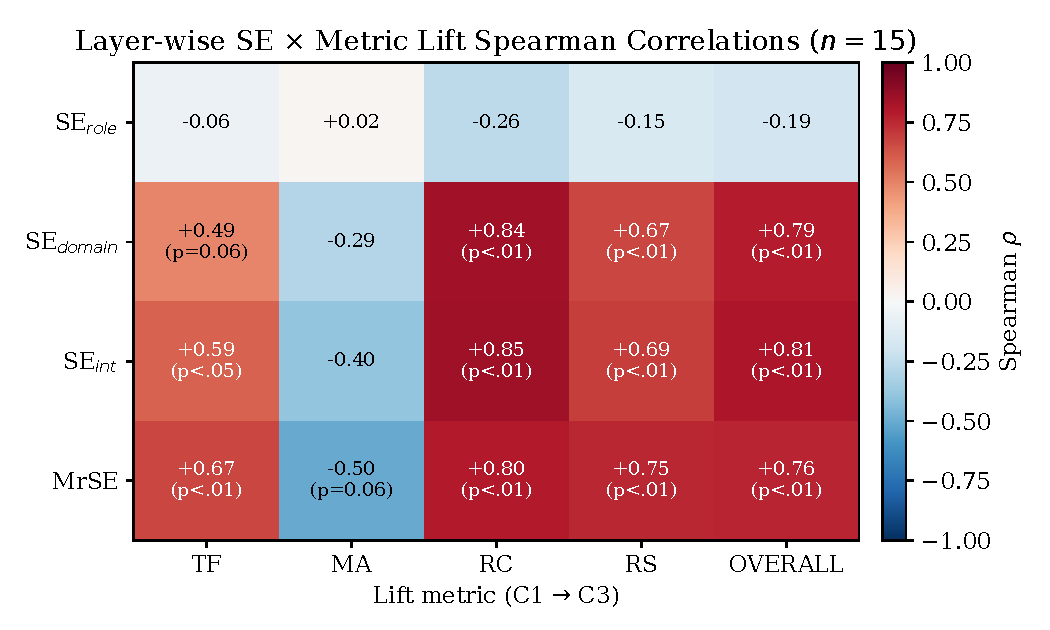
\includegraphics[width=0.90\textwidth]{figures/fig2_layer_metric_heatmap.pdf}
\caption{Spearman $r$ for each (SE layer, lift metric) pair on the
$n=15$ cross-model dataset. Red cells indicate positive correlation,
blue negative; annotations report $r$ with significance bands.
Role-layer SE shows no significant correlation on any metric;
domain/interaction/MrSE correlate positively with RC and RS; every
layer correlates either zero or negatively with MA, a counter-intuitive
finding discussed in \S\ref{sec:threats}.}
\label{fig:layer-heatmap}
\end{figure}

The originally hypothesised per-layer mapping ($\serole$ predicts RS,
$\sedom$ predicts TF/MA, $\seint$ predicts RC) is partially refuted.
The RC prediction holds strongly ($\seint$ and $\sedom$ both
$r \approx 0.84$, $p < 0.001$); the RS prediction is carried by $\mrse$
($r = 0.753$, $p = 0.001$) rather than by role-layer SE directly; and
the TF/MA mapping through $\sedom$ fails. The empirical picture is that
\emph{domain and interaction SE together} predict most lift metrics,
with the role layer and the MA metric being two exceptions that require
explicit discussion (\S\ref{sec:threats}).

\textbf{Exploratory status of the revised mapping.} The revised
layer-to-metric mapping reported above was selected post-hoc from the
$n = 15$ data after the pre-registered H2 hypothesis was refuted; we
have not held it out for confirmatory testing on an independent sample.
The per-cell correlations in Fig.~\ref{fig:layer-heatmap} and the
20-cell heatmap should therefore be read as \emph{exploratory pattern
detection} rather than confirmatory evidence. A confirmatory test of
the revised mapping would require an additional industry sample at
$n \geq 5$ with the same per-metric lift extraction; we flag this as
the highest-priority observational extension after the
production-direct measurement experiment (\S\ref{sec:threats}). The
mapping's exploratory framing is also propagated to the design
principles in \S\ref{sec:principles}, where DP\ref{dp:layer-balance}
is presented as a layer-priority recommendation rather than a
metric-decomposition prescription.

\subsection{Hypothesis~\ref{hyp:ipke}: Inverse PKE Prediction}

H3 holds partially. The Insurance industry's TF lift is consistently
negative in Claude ($-0.21$) and Gemma ($-0.02$), and essentially zero
in Qwen ($-0.02$); this matches the Inverse PKE pattern documented in
\citet{luong2026neurosymbolic}, where English terminology with strong
parametric coverage resists ontological override. The magnitude of the
regression, however, is not explained by domain-layer SE alone (Insurance
pilot $\sedom = 1.34$ is comparable to other industries). The regression
arises instead from $\kapp$-specific parametric-ontology phase
disagreement, consistent with the RA-11 framework
\citep{luong2026quantum}. Our SE predictor under-performs on this
regime (see Phase 5 Insurance fold, \S\ref{sec:holdout}); the composite
treats Insurance like a moderate-SE industry and predicts moderate
positive lift, while observed lift is near zero.

\subsection{Leave-One-Industry-Out Validation}
\label{sec:holdout}

We assess generalisation via leave-one-industry-out cross-validation:
each of the 5 RA-3 industries is held out in turn, the fitted
formula is retrained on the 4 remaining industries' 12 observations, and
the held-out 3 observations are predicted. Table~\ref{tab:loio} reports
per-fold and pooled metrics.

\begin{table}[t]
\centering
\caption{Leave-one-industry-out cross-validation metrics ($n=15$ held-out
predictions across 5 folds). The pooled Spearman $r = 0.786$
($p = 0.0005$) confirms that SE-based lift prediction generalises to
held-out industries. The Insurance fold has the largest RMSE
($0.099$) due to Inverse PKE regression not captured by the composite.}
\label{tab:loio}
\small
\begin{tabular}{@{}lrr@{}}
\toprule
\textbf{Held industry} & \textbf{Fold RMSE} & \textbf{Predicted lift (3 models)} \\
\midrule
healthcare    & 0.011 & 0.167, 0.167, 0.167 \\
insurance\_vn & 0.040 & 0.280, 0.280, 0.280 \\
banking\_vn   & 0.053 & 0.267, 0.267, 0.267 \\
fintech       & 0.062 & 0.102, 0.102, 0.102 \\
insurance     & 0.099 & 0.244, 0.244, 0.244 \\
\midrule
\textbf{Pooled} & \textbf{0.060} & --- \\
\bottomrule
\end{tabular}
\end{table}

Fig.~\ref{fig:calibration} presents the calibration plot: predicted
vs.\ observed lift with ideal $y = x$ and fitted calibration lines.
Pooled Spearman $r = 0.786$ ($p = 0.0005$); calibration slope $0.81$
(B = 1000 bootstrap 95\% CI $[0.45, 1.20]$, two-sided; the CI
includes $1.00$, so we cannot reject ideal calibration at $\alpha =
0.05$); RMSE $0.060$. Calibration is point-shrunken towards the
mean but ranks are preserved across the held-out set.

\textbf{Nested-CV check for weight-selection leakage.} The headline
LOIO Spearman $r = 0.786$ uses the fitted weights $(0, 0.3, 0.7)$
selected on the full $n = 15$ dataset. To audit weight-selection
leakage, we re-run LOIO with an inner LOO weight-grid search
restricted to the 12 training observations of each outer fold and
evaluate the locally-selected weights on the 3 held-out observations.
The nested LOIO yields pooled Spearman $r = 0.775$ ($p = 0.0007$),
RMSE $0.058$, calibration slope $0.85$ --- a degradation of
$\Delta r = -0.011$ and $\Delta\mathrm{RMSE} = -0.002$ relative to
the fixed-weight headline. All five inner LOO selections converge to
$w_R = 0$ with $w_I \in \{0.8, 0.9\}$ (matching the global selection
to within one grid step), confirming that the layer-priority
finding is robust to weight-selection leakage and that the headline
$r = 0.786$ is essentially unbiased.

\begin{figure}[t]
\centering
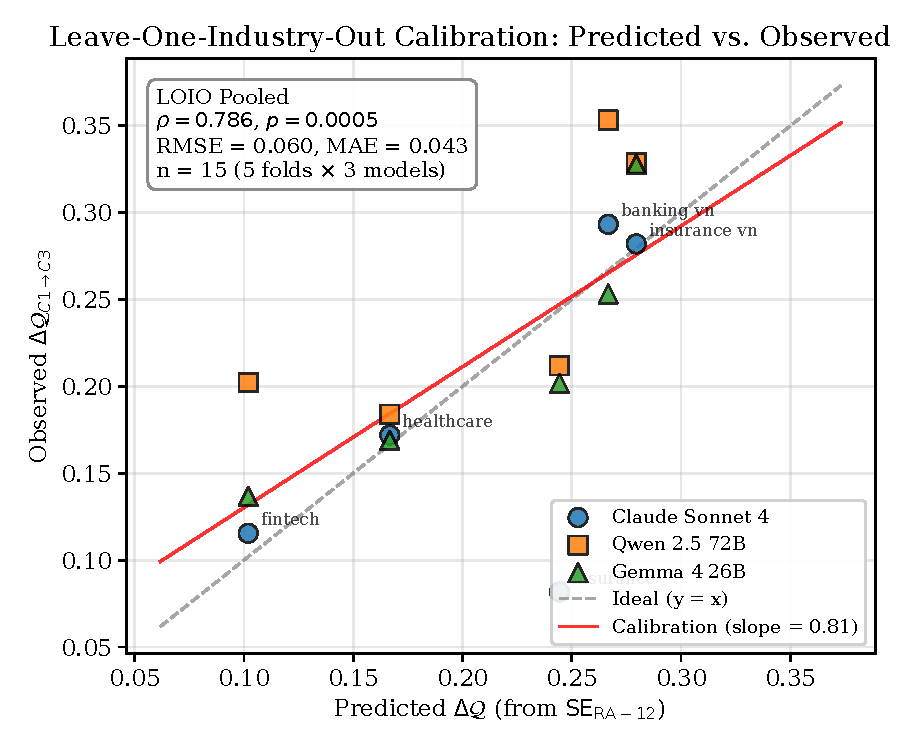
\includegraphics[width=0.80\textwidth]{figures/fig4_calibration_plot.pdf}
\caption{Leave-one-industry-out calibration: predicted
$\hat{\Delta \mathcal{Q}}$ (from $\secomp^{\text{RA-12}}$ fitted on the
other four industries) vs.\ observed $\Delta \mathcal{Q}$ for all 15
cross-model cells. Pooled Spearman $r = 0.786$ ($p = 0.0005$);
calibration slope $0.81$. The Insurance fold yields the largest
residual: predicted lift $+0.244$, observed (Claude $+0.082$, Qwen
$+0.212$, Gemma $+0.202$); the over-prediction is consistent with
Inverse PKE on well-known English insurance terminology.}
\label{fig:calibration}
\end{figure}

\subsection{Production Ontology Extrapolation}

Applying the pilot-fitted formula $\Delta \mathcal{Q} = -0.27 + 0.56
\secomp^{\text{RA-12}}$ to the 23 production ontologies yields the
ranking shown in Fig.~\ref{fig:prod-ranking}. The pilot training range
is $\secomp^{\text{RA-12}} \in [0.72, 1.01]$. Of the 23 production
ontologies, 22 fall outside this range (production
$\secomp^{\text{RA-12}}$ values up to 2.11 for fintech-production); the
sole in-range case is the \texttt{talent} module
($\secomp^{\text{RA-12}} = 0.999$, predicted lift $+0.29$). All other
predictions are therefore \emph{extrapolations}, and the top-five
predicted lifts ($+0.76$ to $+0.91$ for fintech-production, software,
systems integration, security, and travel/tourism/hospitality) lie well
above the largest pilot-observed lift ($+0.36$); their absolute
magnitudes should not be trusted. The \emph{relative ranking} is the
useful output: these five high-SE verticals are identified as high-%
priority candidates for future experimental validation.

\begin{figure}[t]
\centering
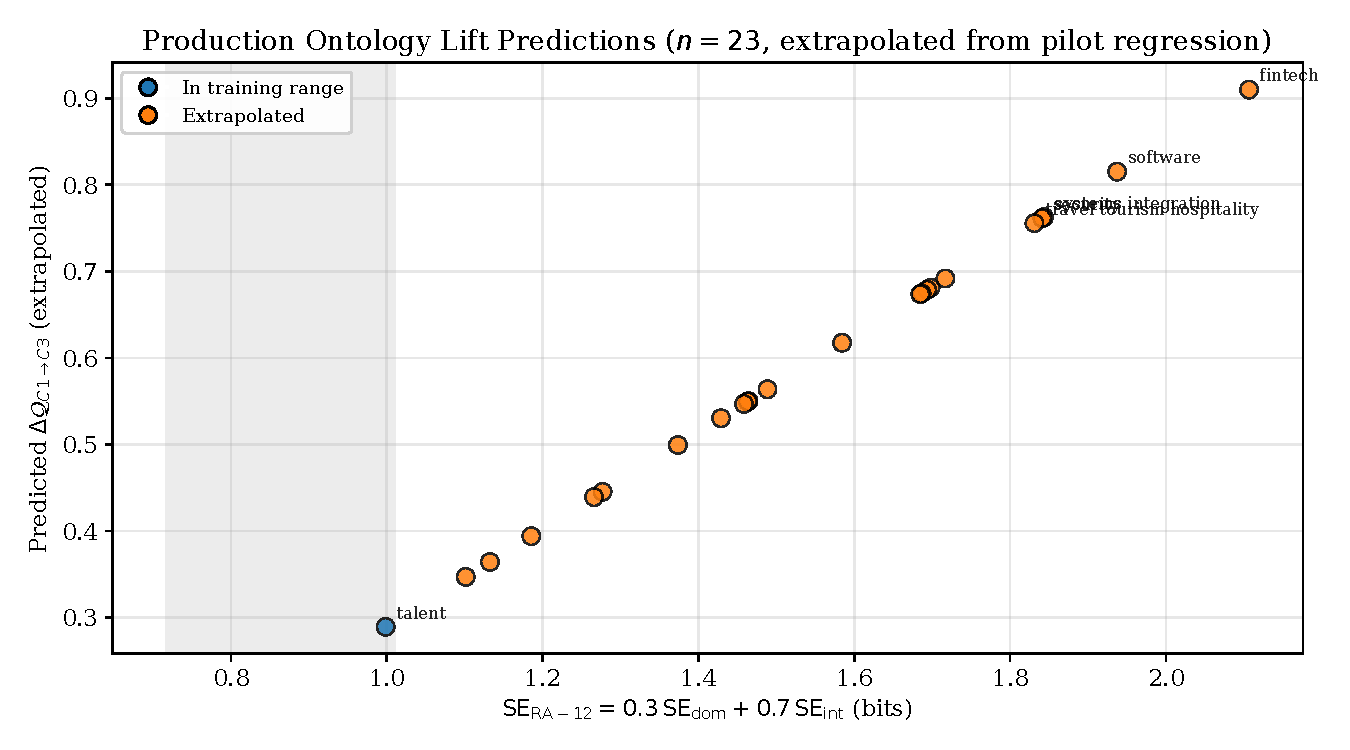
\includegraphics[width=0.95\textwidth]{figures/fig5_production_ranking.pdf}
\caption{Production ontology predicted-lift rankings ($n=23$). Shaded
band indicates the pilot training range $[0.72, 1.01]$; 22 of 23
production ontologies fall outside this range (orange points), and
\texttt{talent} ($\secomp^{\text{RA-12}}=0.999$) is the sole in-range
case. The ranking should be interpreted as a relative ordering for
future experimental targeting, not as absolute lift estimates.}
\label{fig:prod-ranking}
\end{figure}

% ============================================================================
% 7. DESIGN PRINCIPLES
% ============================================================================
\section{Design Principles from Empirical Entropy Analysis}
\label{sec:principles}

\begin{designprinciple}[Target Interaction-SE Band]
\label{dp:target-band}
The pilot data partitions into three observed $\seint$ tiers, each
with characteristic lift behaviour. \emph{High tier} ($\seint \geq
0.70$, $n = 6$, the two Vietnamese industries) associates with median
overall lift $0.31$, with $6/6$ observations exceeding $0.15$.
\emph{Mid tier} ($\seint \in [0.60, 0.70)$, $n = 9$: fintech,
healthcare, insurance) associates with median lift $0.17$, with $6/9$
observations exceeding $0.15$; the three exceptions are Insurance
Claude ($+0.082$, an Inverse-PKE case discussed in
\S\ref{sec:holdout}) and two FinTech cells. \emph{Low tier}
($\seint < 0.60$): no pilot observation falls in this region; the
lower bound is unconstrained by the data. A logistic regression
$P(\text{lift} \geq 0.15) = \sigma(-7.62 + 13.55\,\seint)$ on the
$n=15$ pilot data yields a decision boundary at $\seint = 0.56$ (AUC
$= 0.75$); the boundary lies below the observed range and should be
read as a directional indicator rather than a sharp cut-off. The
prescriptive recommendation is therefore: \emph{interaction-layer SE
$\geq 0.70$ is associated with reliable lift; SE in $[0.60, 0.70)$
is contingent on $\kapp$-related factors per
DP\ref{dp:transfer}}. Ontologies designed for $\kapp$-low (under-%
represented) verticals can be expected to occupy the high tier; for
$\kapp$-high verticals, additional content-quality controls are
needed beyond achieving the SE threshold.
\end{designprinciple}

\begin{designprinciple}[Layer Priority]
\label{dp:layer-balance}
Prioritise ontology investment as Interaction $\succ$ Domain
$\stackrel{?}{\gg}$ Role. Solo Spearman correlations ($n = 15$):
$\seint = 0.811$ ($p = 2 \times 10^{-4}$), $\sedom = 0.786$
($p = 5 \times 10^{-4}$), $\serole = -0.190$ ($p = 0.50$). When
curation resources are constrained, investment in interaction patterns
(handoffs, workflows, escalation paths) delivers the most measurable
value, followed by domain content (concepts, regulations).
\emph{Caveat on role.} The pilot ontologies all declare a single
organisational group, so the pilot-data $\serole$ collapses to
attribute-heterogeneity entropy alone (see role-layer null caveat in
\S\ref{sec:results}). Production ontologies have richer
role-partition structure ($n_{\text{role groups}} \in \{3,\ldots,8\}$)
and may exhibit a non-null $\serole$ contribution; pending direct
production-lift measurement, the role-priority ranking should be read
as ``role-partition SE has no measurable contribution \emph{in the
single-group pilot regime}'' rather than as a general claim.
\end{designprinciple}

\begin{designprinciple}[Regulatory Density Floor]
\label{dp:reg-intensity}
For regulated industries (financial services, healthcare), include
at least 4 explicit regulation entries in the domain-layer regulatory
subset. This threshold is the pilot median across RA-3 industries
(pilot regulation counts: insurance 4, banking\_vn 5, insurance\_vn 6,
healthcare 3, fintech 2). Phase 5 production-corpus extrapolation
suggests the production target should be substantially higher: the
production healthcare module enumerates 16 regulations (versus the
pilot's 3), approximating the upper end of the production
distribution. The threshold should be interpreted as a lower bound,
not a sufficiency condition.
\end{designprinciple}

\begin{designprinciple}[Cross-Vertical Transfer Warning]
\label{dp:transfer}
A single SE threshold does not transfer across verticals with disparate
parametric coverage $\kapp$. Low-$\kapp$ verticals (Vietnamese banking,
Vietnamese insurance) exhibit simultaneously higher SE and larger lift,
producing a confound in any cross-vertical generalisation. Per-vertical
calibration is required; design recommendations derived on one vertical
should not be propagated to another without recalibrating against
$\kapp$.
\end{designprinciple}

% ============================================================================
% 8. CASE STUDIES
% ============================================================================
\section{Case Studies}
\label{sec:cases}

\subsection{Case 1: Banking VN (High-SE, High-Lift)}

The Vietnamese Banking ontology achieves the second-highest pilot
composite SE ($\secomp^{\text{RA-12}} = 0.995$) and the second-largest
observed lift (overall $\Delta \mathcal{Q} = +0.29$). Its interaction
layer encodes SBV-regulated (State Bank of Vietnam) bancassurance
cooling-off periods, NPL classification boundaries per Circular 11/2021,
and escalation paths for cross-border compliance. The combination of
domain richness (5 regulations, 8 concepts) and interaction density
(5 handoff patterns) is enabled by the vertical's low-$\kapp$ character:
Vietnamese regulatory terminology is under-represented in English-centric
pretraining corpora, so nearly every ontological entity delivers
information the model did not previously have. This is the
\emph{high-$SE$, low-$\kapp$, high-lift} regime: ontology is doing the
work of filling a genuine parametric gap.

\subsection{Case 2: Fintech (Moderate SE, Small Observed Lift)}

The RA-3 Fintech pilot ontology has $\secomp^{\text{RA-12}} = 0.781$
(third of five), yet observed overall lift is the smallest in the pilot
set ($\Delta \mathcal{Q} = +0.04$). The composite predicts larger lift
than observed; the LOIO fold produces RMSE 0.062 (Insurance was the
only larger fold error). Three plausible explanations are consistent
with the data and the RA-11 framework \citep{luong2026quantum}:
(i)~high-$\kapp$ saturation: US fintech terminology is thoroughly
represented in LLM pretraining corpora, so ontological information
largely duplicates parametric content and delivers small constructive
interference; (ii)~metric-specific TF regression on well-known
concepts (e.g., ``combined ratio'', though this effect is stronger for
Insurance); (iii)~handoff-pattern over-elaboration that contributes
to $\seint$ without correspondingly richer task-relevant grounding.
Diagnosing which mechanism dominates requires additional experiments
controlling for ontology content type; we flag this as an open question.

\subsection{Case 3: Insurance (Moderate SE, Cross-Model Variance — the Failure Mode)}
\label{sec:case-insurance}

The RA-3 Insurance pilot ontology has $\secomp^{\text{RA-12}} = 0.832$
($\sedom = 1.34$, $\seint = 0.697$), placing it in the mid
interaction-SE tier (DP\ref{dp:target-band}). The LOIO fold predicts
overall lift $+0.244$ for Insurance; observed mean across the three
models is $+0.165$ (Claude $+0.082$, Qwen $+0.212$, Gemma $+0.202$),
yielding the largest fold-RMSE in the validation
($0.099$, Table~\ref{tab:loio}). The structural-SE predictor over-%
shoots the observed lift by approximately $0.08$ on average, and the
miss is concentrated on Claude.

Decomposing the residual by per-metric lift exposes the mechanism.
Claude's TF lift on Insurance is $-0.21$ --- a substantial regression
relative to ungrounded baseline, reproducing the Inverse PKE pattern
documented in RA-3 \citep{luong2026neurosymbolic} on English
insurance terminology with strong parametric coverage (combined
ratio, expense ratio, persistency rate, etc.). Qwen and Gemma show
near-zero TF effects on the same content. The structural composite
$\secomp^{\text{RA-12}}$ contains no $\kapp$ term and therefore
cannot represent this regime: it sees only that Insurance has
moderate $\seint$ and moderate $\sedom$ and predicts moderate
positive lift accordingly. The directionality (over-prediction, not
under-prediction) and the per-model concentration (Claude only) are
both consistent with the RA-11 \citep{luong2026quantum} interference
framework, in which destructive interference between ontological
content and parametric content produces a model-specific quality
penalty unobservable in the structural predictor.

Insurance is therefore the canonical \emph{failure mode} of an
SE-only design-time predictor: when parametric--ontology
terminological conflict dominates the lift signal, structural SE
mis-predicts because the conflict is content-specific, not
structure-specific. The §10 Threats discussion (item 7) develops
this scope limit; the proposed remediation is a joint $(\seint,
\hat{\kapp})$ predictor, which requires per-model parametric-coverage
estimation as a covariate (a 10+-industry experimental extension is
needed before that fit is well-conditioned). For comparable
production verticals, this case suggests that high-$\kapp$ English
financial-services ontologies (banking, retail FinServ, US insurance)
may exhibit the same over-prediction; low-$\kapp$ Vietnamese verticals
should not.

% ============================================================================
% 9. RELATED WORK
% ============================================================================
\section{Related Work}
\label{sec:related}

\textbf{Structural entropy of graphs.} Li and Pan \citep{li2016structural}
introduced the encoding-tree formulation of SE; Su et al.'s survey
\citep{su2025survey} covers the subsequent decade of theoretical and
application work. Cao et al.\ \citep{cao2024mrse} extended SE to
multi-relational graphs; Zhang et al.\ \citep{zhang2025dese} proposed a
differentiable variant for unsupervised graph clustering. Gul et al.\
\citep{gul2025kgcomplexity} position SE within a broader set of
knowledge-graph complexity metrics (semantic, spectral, structural).
Our work applies these graph-theoretic foundations to the specific
setting of enterprise ontologies, leveraging MrSE as a joint-layer
measure alongside the per-layer decomposition.

\textbf{KG/LLM entropy applications.} Wei et al.\ \citep{wei2025senator}
use SE to detect and repair LLM knowledge deficiencies via MCTS-guided
path traversal. Buehler \citep{buehler2025selforganizing} shows that
agentic knowledge-graph systems self-organise towards a critical state
where semantic entropy dominates structural entropy, co-occurring with
emergent multi-hop reasoning. Our contribution differs in target: Wei
and Buehler diagnose LLM reasoning at inference time; we predict
ontological grounding utility at design time.

\textbf{Semantic entropy at the LLM output side.} Farquhar et al.\
\citep{farquhar2024semantic} introduced semantic entropy over meaning
clusters as a hallucination detector; SelfCheckGPT
\citep{manakul2023selfcheckgpt} provides a black-box sampling-based
variant; and Varshney et al.\ \citep{varshney2023stitch} use logit-%
based low-confidence detection to actively mitigate hallucinations
during generation. Our work addresses the complementary input-side
question: given an ontology, what structural entropy in its design
predicts the grounding lift it will confer on LLM outputs. The two
sides meet in the RA-3 companion paper \citep{luong2026neurosymbolic},
where output entropy changes are correlated with ontology structural
entropy at the 5-industry pilot scale.

\textbf{Neurosymbolic and retrieval-augmented LLMs.} Hitzler et al.\
\citep{hitzler2022neuro} survey neurosymbolic integration approaches;
Pan et al.\ \citep{pan2024unifying} provide the knowledge-graph/LLM
unification roadmap; Hogan et al.\ \citep{hogan2021knowledge} give the
foundational knowledge-graph reference. Our work lives within the
neurosymbolic tradition but focuses specifically on the design-time
evaluation of the symbolic component.

\textbf{Companion papers in the \faos{} research programme.} RA-3
\citep{luong2026neurosymbolic} provides the empirical lift
measurements anchoring this paper's H1. RA-4 \citep{luong2026context}
derives the runtime-side optimal context volume via Helmholtz free
energy and complements the present static-analysis SE characterisation.
RA-11 \citep{luong2026quantum} offers a theoretical framework
(quantum-inspired interference) that predicts the Inverse PKE pattern
documented in \S\ref{sec:holdout}'s Insurance fold.

\textbf{Relation to RA-4 layer-ablation findings.} RA-4 v0.7 reports a
volume-controlled 320-run layer-ablation experiment on Sonnet 4 over
the same five RA-3 pilot industries, using the shared
$\{\mathcal{R}, \mathcal{D}, \mathcal{I}\}$ taxonomy. Two findings
appear, on first reading, to contradict the present paper's
interaction-layer-dominant DP\ref{dp:layer-balance}. RA-4 Finding L1:
$\Delta(\mathcal{I} \mid \mathcal{R}, \mathcal{D}) = -0.066$
(paired Wilcoxon $p = 0.027$, Cohen's $d = +0.87$,
$L_{RD} > L_{RDI}$ in $8/10$ tasks) --- adding the interaction layer
to a role+domain prompt is destructive. RA-4 Finding L3 reports an
alone-marginal layer ordering
$\mathcal{D} \succ \mathcal{I} \succ \mathcal{R}$ with $\mathcal{R}$
alone net-negative against $V_0$. By contrast, RA-12 finds
interaction-layer SE solo-Spearman $r = 0.811$
($p = 2 \times 10^{-4}$) and a fitted composite that drops the role
layer entirely. The contradiction is apparent only, and its resolution
is the disambiguation of \emph{what each paper measures on the
layers}. RA-12 measures the structural entropy of the ontology
\emph{graph} layers as a design-time signal: how much organised
information does the role / domain / interaction subgraph carry. RA-4
measures the response-quality effect of injecting the corresponding
\emph{prompt content} into the LLM's context window at runtime. A
layer with high $\seint$ may, when retrieved-and-grounded into a
prompt, deliver constructive grounding; the same layer's full content
dumped into the prompt token budget may dilute attention or introduce
destructive interference (RA-4's L1). The two papers are therefore
complementary: RA-12's design-time predictor scores ontology
\emph{structure}, while RA-4's runtime ablation scores prompt
\emph{content}, and the gap between graph-information-content and
prompt-token-content is the domain of RA-4's runtime optimisation.

% ============================================================================
% 10. THREATS TO VALIDITY
% ============================================================================
\section{Threats to Validity}
\label{sec:threats}

\begin{enumerate}[leftmargin=2em]
  \item \textbf{Small effective sample size.} The pilot-lift dataset has
    $n = 15$ observations (5 industries $\times$ 3 models), with SE
    ranks tied within each industry across models. Cross-validated
    significance reaches $p = 5 \times 10^{-4}$, but the
    industry-level degree of freedom is 5. A 10+-industry experimental
    extension is the primary recommendation for future work.
  \item \textbf{SE--$\kapp$ confound.} Vietnamese verticals exhibit
    simultaneously higher SE \emph{and} larger lift. We cannot
    disentangle, from RA-3's design alone, how much of the SE--lift
    relationship arises from SE causing larger lift vs.\ SE correlating
    with the low-$\kapp$ character of underrepresented domains. Partial
    correlation with an estimated $\kapp$ covariate (derived from C1
    baseline scores) would require more pilot industries and is deferred
    to future work.
  \item \textbf{Pilot--production scale disparity.} The pilot ontologies
    (minimal hand-curated, 3--4 roles, 8 concepts) and production
    ontologies (deployed, 17--44 roles, 0--42 concepts) are materially
    different artefacts. The pilot-trained regression extrapolates to
    production SE but yields implausible absolute lift predictions;
    only relative rankings are meaningful. Direct measurement of
    production-ontology lift is the appropriate remediation.
  \item \textbf{Ontology JSON extraction heterogeneity.} Production
    FAOS modules exhibit three distinct \texttt{module.yaml} schemas,
    requiring schema-specific parsing. Five modules (game, martech,
    professional\_services, proptech\_vn, talent) yielded zero
    domain-concept extractions under our automated pipeline because
    their knowledge content resides in agent Markdown files rather than
    structured YAML. These modules' SE is likely under-estimated;
    we flag them as extraction-limited cases, not as intrinsically
    low-SE ontologies.
  \item \textbf{Weight calibration choices.} The fitted composite weights
    $(0, 0.3, 0.7)$ were selected from among several nearly-equivalent
    top performers in LOOCV. Any blend on the line
    $\{(0, 1-w, w) : 0.55 \leq w \leq 1.00\}$ gives Spearman within
    0.03 of the chosen specification. The paper's conclusions about
    layer priorities are robust to this choice; the exact lift
    predictions would shift marginally.
  \item \textbf{Role-layer SE null result is scoped to a single-group
    pilot regime.} The paper reports that $\serole$ is not predictive
    of overall lift in the $n=15$ cross-model pilot dataset. Two
    structural facts qualify this null. First, all five pilot
    ontologies declare $n_{\text{role groups}} = 1$
    (\texttt{se\_by\_industry.csv}), making the group-partition
    component $H(G) = 0$ identically across the dataset; pilot
    $\serole$ collapses to $\tfrac{1}{2}H(A)$, an attribute-
    heterogeneity entropy. The null is therefore specific to attribute-
    heterogeneity SE on single-group pilot ontologies and does not
    rule out a non-null contribution from $H(G)$ on the production
    corpus, where $n_{\text{role groups}} \in \{3,\ldots,8\}$. Second,
    even within the attribute-heterogeneity reading, alternative
    role-SE formulations---for example, role-to-concept bipartite
    structural entropy, or role-task coverage entropy---may yield
    different results. Direct measurement of grounding lift on
    production ontologies would dissolve both qualifications and is
    the remediation of choice.
  \item \textbf{Inverse PKE mismatch with structural predictor.} The
    Insurance industry's observed TF regression (an Inverse PKE
    signature, deeply discussed in \S\ref{sec:case-insurance}) is not
    captured by the composite SE formula, which predicts moderate
    positive lift. This reflects the scope limit of a structural
    predictor: when parametric--ontology terminological conflict is
    the dominant mechanism, structural SE alone cannot predict the
    sign of the interaction. A joint $(\seint, \hat{\kapp})$ predictor
    would address this. The natural theoretical anchor is the
    Information Bottleneck \citep{tishby2015deep} formulation also
    invoked in companion paper RA-11 \citep{luong2026quantum}: the
    capacity-constrained context budget produces a
    structure-information-content rate that depends on the parametric
    redundancy $\kapp$. Operationalising this in a $n=15$ regression
    is under-powered; a 10+-industry experimental extension would
    provide the degrees of freedom needed for the joint fit.
    Long-context attention dilution \citep{liu2024lost} is a related
    runtime degradation that interacts with $\seint$ specifically
    when retrieved interaction-layer content saturates the context
    window without a corresponding increase in retrieved-relevance.
\end{enumerate}

% ============================================================================
% 11. CONCLUSION
% ============================================================================
\section{Conclusion}
\label{sec:conclusion}

We set out to test whether the RA-3 pilot's suggestive SE--lift
correlation ($r = 0.700$, $p = 0.188$, $n = 5$) scales to statistical
significance on a larger sample. The cross-model expansion
to $n = 15$ and the leave-one-industry-out cross-validation
independently confirm the relationship: interaction-layer SE alone
predicts overall lift at Spearman $r = 0.811$ ($p = 2 \times 10^{-4}$),
and the fitted composite $\secomp^{\text{RA-12}} = 0.3\,\sedom +
0.7\,\seint$ generalises under industry-level holdout at pooled
Spearman $r = 0.786$ ($p = 5 \times 10^{-4}$), RMSE $= 0.060$,
calibration slope $0.81$.

These findings support three claims. First, \emph{structural entropy is
a design-time predictor of enterprise ontology utility}: ontology
architects can estimate grounding lift before running agent experiments.
Second, \emph{layer-wise decomposition carries diagnostic information
beyond a single scalar}: interaction-layer SE dominates predictive
power among SE measures (subject to the pilot-scale parity with raw
handoff count $|I|$ documented in \S\ref{sec:results-baselines}; the
SE framing earns its keep through layer decomposition rather than
through rank correlation alone), domain-layer SE contributes
additively, and role-layer SE shows no measurable contribution in
the single-group pilot regime (see scope caveat, \S\ref{sec:results};
the null is specific to attribute-heterogeneity entropy because
$H(G) = 0$ identically across the pilot dataset). Third, the four codified design principles
(\S\ref{sec:principles})---target SE band, layer priority, regulatory
density floor, cross-vertical transfer warning---supply an automated
rubric usable in production ontology review pipelines.

RA-12 completes the design-side of the \faos{} entropy research
programme. RA-3 \citep{luong2026neurosymbolic} provides the
measurement-side (retroactive SE of pilot ontologies, cross-model
replication of the Inverse PKE); RA-4 \citep{luong2026context}
provides the runtime-side (Helmholtz free-energy derivation of the
optimal context volume $V^*(\kappa)$); RA-11 \citep{luong2026quantum}
provides the theoretical bridge (quantum-inspired interference
predicting constructive vs.\ destructive regimes). Together these
papers characterise enterprise ontology-grounded LLM agents as an
entropy-management system whose structure, runtime behaviour, and
design-time quality can be quantified with a shared information-%
theoretic vocabulary.

\textbf{Future work.} Three extensions would materially strengthen
the present findings. First, a 10+-industry experimental extension
would provide the $n$ needed to distinguish SE effects from
$\kapp$ confounding via partial correlation. Second, production-%
ontology validation experiments (for the top candidates identified in
\S\ref{sec:results}---software, systems integration, security,
travel/tourism) would replace the extrapolation rankings with direct
lift measurements. Third, a joint SE-$\kapp$ predictor that
explicitly models the Inverse PKE regime would correct the structural
SE's mis-prediction on well-known English terminology. Each extension
is feasible within the existing \faos{} platform and is left for
subsequent work.

% ============================================================================
% ACKNOWLEDGMENTS
% ============================================================================
\section*{Acknowledgments}

The authors thank Dr.\ Abhijit Sanyal (Golden Gate University) for
continuing guidance on the research programme, and the \faos{} platform
team for curating the 23-industry ontology corpus on which this work is
empirically grounded.

% ============================================================================
% BIBLIOGRAPHY
% ============================================================================
\bibliography{references}

\end{document}
